\chapter{Five Lessons From Multi-Millionaire Interviews}

This chapter follows a School of Hard Knocks entrepreneurship interview curated by LazyingArt LLC through Video2Book. The speaker presents five lessons that he says recur across interviews with more than a thousand multi-millionaires. We will treat that statement as reported interview context, not as a statistical proof. What matters for the notes is the sequence of mechanisms: risk creates learning, passion needs a monetization path, starting sooner creates feedback, networks create access, and earned money has to be converted into assets if it is to work beyond the original labor.

\section{The Interview Claim and the Five-Lesson Frame}

The lecture opens with a claim of breadth: the speaker says he has interviewed over a thousand multi-millionaires and is now distilling the top five lessons he has learned from those conversations. That opening sets the epistemic level of the chapter. We are not reading a controlled study or a formal economic model. We are reading a compressed set of interview-derived observations.

So we should keep three layers separate:

\begin{itemize}
\item the anecdote: what the speaker says he has heard repeatedly;
\item the claim: what action the lesson recommends;
\item the mechanism: why that action might change outcomes.
\end{itemize}

The whole lecture can be read as a feedback system. The speaker's five lessons are not isolated slogans. They are successive ways of strengthening the loop

\begin{equation}
\text{action}
\longrightarrow
\text{feedback}
\longrightarrow
\text{learning}
\longrightarrow
\text{better action}.
\end{equation}

The first lesson, risk, starts the loop. The second lesson asks what kind of work deserves that risk. The third asks when to begin. The fourth asks who should surround the effort. The fifth asks what to do with the money if the effort begins to work.

\section{Risk, Failure, and the Comfort Zone}

The speaker begins the numbered lessons with risk. He says he has heard, again and again, that young people should not be afraid to take risks. The obstacle appears immediately: people are afraid of failing, so they play safe. The contrast is between the safety of avoiding loss and the ambition of reaching the top of an industry.

The lecture does not claim that risk is automatically rewarded. Its claim is subtler. Risk matters because it exposes the entrepreneur to information that cannot be obtained from a protected position. In its simplest form, the mechanism is

\begin{equation}
\text{risk}
\longrightarrow
\text{possible failure}
\longrightarrow
\text{learning}
\longrightarrow
\text{growth}.
\end{equation}

But one step must be made explicit. Failure by itself is not the teacher. The response to failure is the teacher:

\begin{equation}
\text{failure}+\text{constructive response}
\longrightarrow
\text{usable information}.
\end{equation}

This is why the lecture spends time on getting back up, learning from mistakes, and continuing. The speaker is not romanticizing failure. He is treating it as part of an update process.

\subsection{Question \& Answer}

\paragraph{Question.}
If taking risks makes failure more likely, why take the risk?

\paragraph{Answer.}
Because the final object is not the single attempt. The final object is the sequence of attempts. Let \(L_n\) denote what has been learned after the \(n\)-th attempt. A simple update rule is

\begin{equation}
L_{n+1}=L_n+\Delta L_n,
\end{equation}

where \(\Delta L_n\) is the useful lesson extracted from the attempt. A protected non-attempt may avoid embarrassment, but it often gives

\begin{equation}
\Delta L_n \approx 0.
\end{equation}

The point is not that every risk pays immediately. The point is that the person who keeps acting and extracting information has more opportunities to improve the next action.

The comfort zone now has a practical definition. It is the region where the feedback loop is weak because action is too protected to reveal much. The speaker says that discomfort forces growth: new skills, changed habits, adaptation, and learning the details of unfamiliar situations.

\begin{figure}
\centering
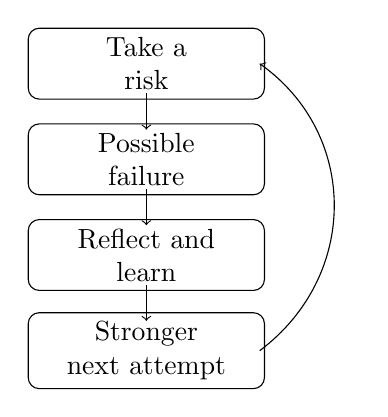
\begin{tikzpicture}[scale=0.9]
\node[draw, rounded corners, align=center, minimum width=3.0cm, minimum height=0.8cm] at (0,0) {Take a\\risk};
\node[draw, rounded corners, align=center, minimum width=3.0cm, minimum height=0.8cm] at (0,-1.35) {Possible\\failure};
\node[draw, rounded corners, align=center, minimum width=3.0cm, minimum height=0.8cm] at (0,-2.70) {Reflect and\\learn};
\node[draw, rounded corners, align=center, minimum width=3.0cm, minimum height=0.8cm] at (0,-4.05) {Stronger\\next attempt};
\draw[->] (0,-0.42) -- (0,-0.93);
\draw[->] (0,-1.77) -- (0,-2.28);
\draw[->] (0,-3.12) -- (0,-3.63);
\draw[->] (1.6,-4.05) .. controls (3.0,-3.0) and (3.0,-1.0) .. (1.6,0);
\end{tikzpicture}
\end{figure}

The diagram is a conceptual reconstruction of the spoken loop. No board diagram was retained for this lecture.

\section{Passion Must Meet Monetization}

The second lesson changes the question. Once we accept that action requires risk, we still need to decide what to act on. The speaker says to follow passion, but he does not leave the point there. He says to align passion with what can be monetized.

That qualification is important. The lecture's examples are broad: music, coding, sports, content, services, and products. The common structure is not merely that the person cares. It is that the care is connected to a channel through which value can be created and exchanged.

The weak version would be

\begin{equation}
\text{passion}\longrightarrow\text{business}.
\end{equation}

The lecture's stronger version is

\begin{equation}
\text{passion}+\text{monetization path}
\longrightarrow
\text{commercial effort}.
\end{equation}

\begin{definition}
A monetizable passion is an activity the person cares about, joined to a concrete channel through which that activity can create value for others and receive payment, attention, or opportunity in return.
\end{definition}

The speaker also warns against chasing work only because it seems profitable in the short run. Work done only for apparent short-term gains may not carry enough energy to sustain the effort. Work done only from feeling may never become a business. The entrepreneurial target is the overlap:

\begin{equation}
\text{entrepreneurial fit}
=
\text{personal energy}
\cap
\text{market demand}.
\end{equation}

This is a compact reconstruction, not a literal formula from the video, but it preserves the two-sided logic of the transcript.

\section{Start Sooner, Before the Idea Becomes Delay}

The third lesson follows from the second. If there is a passion and a possible monetization route, the next issue is timing. The speaker gives a familiar sequence: someone says they will build a business, start a podcast, or open a store; then the plan moves to next month, then six months, then a year, and finally nothing happens.

The mathematical idea is opportunity cost. Delay is not empty time. It is time in which feedback could have been gathered but was not. If \(F(t;s)\) denotes the accumulated feedback by time \(t\) from a project started at time \(s\), then a cautious model is

\begin{equation}
F(t;s)=\int_s^t f(\tau)\,d\tau,
\end{equation}

where \(f(\tau)\) is the rate at which real action produces usable feedback. If two people face the same feedback rate but one starts later, then

\begin{equation}
s_2>s_1
\quad\Longrightarrow\quad
F(t;s_2)\leq F(t;s_1).
\end{equation}

This calculus is a standard reconstruction. The spoken point is simpler: starting sooner gives the project more chances to meet reality.

\subsection{Question \& Answer}

\paragraph{Question.}
What makes waiting costly if the idea can still be started later?

\paragraph{Answer.}
The idea may survive, but the learning has not happened. The speaker's worry is not only that a calendar date moves. It is that the project has not been exposed to customers, viewers, buyers, mentors, mistakes, or market response.

We can write the project as two coupled updates:

\begin{align}
I_{n+1} &= I_n+\Delta I_n,\\
A_{n+1} &= A_n+\Delta A_n.
\end{align}

Here \(I_n\) is information about the market, and \(A_n\) is ability. The increments \(\Delta I_n\) and \(\Delta A_n\) usually require attempts. If the entrepreneur only plans, then both increments remain small. Starting sooner matters because action begins the update process.

This is why the speaker says the third lesson goes hand in hand with the previous one. Passion supplies energy, but starting converts that energy into observation.

\section{Network as a Form of Leverage}

The fourth lesson widens the frame from the individual to the surrounding system. The speaker says to build a network, surround yourself with like-minded people, find mentors, and learn from people who have already done what you want to do. He also notes that entrepreneurship can become lonely, so the network is both informational and emotional.

The word network contains several objects:

\begin{itemize}
\item mentors who have already reached the desired point;
\item peers with similar ambitions;
\item supporters who encourage the work;
\item critics who can correct the work constructively;
\item contacts found through local events, conventions, and industry gatherings.
\end{itemize}

The speaker then connects this lesson back to the first one. His platform reached out to multi-millionaires and business owners. Sometimes the ask was small: ten or fifteen minutes, lunch, or a brief conversation. That is the bridge between risk and network. Outreach itself is an uncomfortable action, but it may create access.

A compact model is

\begin{equation}
\text{network value}
\approx
\text{access}
+
\text{information}
+
\text{accountability}.
\end{equation}

The only numerical detail in this section is modest but concrete: even \(10\) or \(15\) minutes with the right person may carry value. We should not inflate that into a universal rule. The point is that a short contact can transmit context that would otherwise take much longer to discover.

\begin{figure}
\centering
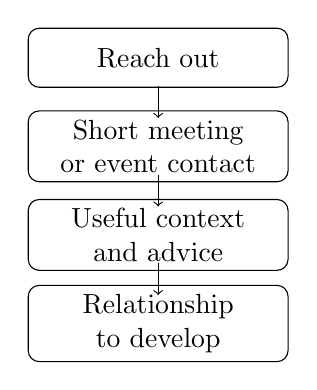
\begin{tikzpicture}[scale=0.9]
\node[draw, rounded corners, align=center, minimum width=3.3cm, minimum height=0.75cm] at (0,0) {Reach out};
\node[draw, rounded corners, align=center, minimum width=3.3cm, minimum height=0.75cm] at (0,-1.25) {Short meeting\\or event contact};
\node[draw, rounded corners, align=center, minimum width=3.3cm, minimum height=0.75cm] at (0,-2.50) {Useful context\\and advice};
\node[draw, rounded corners, align=center, minimum width=3.3cm, minimum height=0.75cm] at (0,-3.75) {Relationship\\to develop};
\draw[->] (0,-0.40) -- (0,-0.85);
\draw[->] (0,-1.65) -- (0,-2.10);
\draw[->] (0,-2.90) -- (0,-3.35);
\end{tikzpicture}
\end{figure}

The order in the lecture should be preserved. The speaker does not jump from networking to events. He first talks about like-minded people, then mentors, then support systems, then constructive criticism, then direct outreach, and finally local community events. The motion is from inner circle to experienced guides to active public contact.

\section{Let Money Work Through Assets}

The final lesson shifts from earning to ownership. The speaker says that multi-millionaires did not simply let money sit in the bank, nor did they spend all of it. They took money earned from careers or businesses and put it into assets: real estate, stocks, markets, and, in the current environment he names, cryptocurrency.

The caution is central. These examples are not promises. They are the categories the speaker lists when describing how money can be made to work. The contrast is

\begin{equation}
\text{idle cash}
\quad\hbox{versus}\quad
\text{assets with possible appreciation}.
\end{equation}

Let \(\pi\) denote inflation and \(y_{\text{bank}}\) the yield on bank deposits. Idle cash loses purchasing power when

\begin{equation}
\pi>y_{\text{bank}}.
\end{equation}

Equivalently, the approximate real return on the cash position is

\begin{equation}
r_{\text{real}}\approx y_{\text{bank}}-\pi.
\end{equation}

That is the standard financial form of the transcript's statement that money sitting in the bank can go down in value over time because of inflation.

For an asset that appreciates at rate \(r\), a simple compounding model is

\begin{equation}
V_t=V_0(1+r)^t,
\end{equation}

where \(V_0\) is the initial value and \(V_t\) is the value after \(t\) periods. This is only a model of possible appreciation. The lecture does not say that every asset appreciates, and the notes should not imply that \(r\) is guaranteed positive.

\paragraph{Worked example.}
Suppose bank deposits yield \(y_{\text{bank}}=1\%\), while inflation is \(\pi=4\%\). Then the approximate real return is

\begin{equation}
r_{\text{real}}\approx 1\%-4\%=-3\%.
\end{equation}

So the nominal balance may look stable while purchasing power declines. Now suppose an asset grows at \(r=5\%\) for three periods. The simple model gives

\begin{align}
V_3 &= V_0(1.05)^3,\\
    &\approx 1.158V_0.
\end{align}

The example is not investment advice. It illustrates the distinction the speaker is making: idle money and allocated money follow different dynamics.

\begin{figure}
\centering
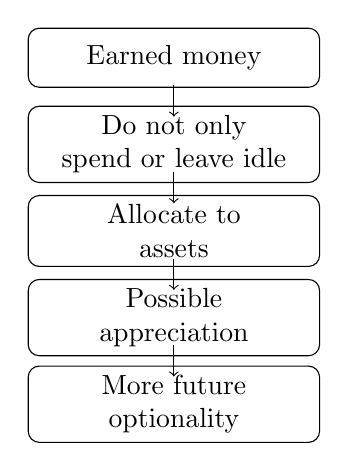
\begin{tikzpicture}[scale=0.88]
\node[draw, rounded corners, align=center, minimum width=3.7cm, minimum height=0.75cm] at (0,0) {Earned money};
\node[draw, rounded corners, align=center, minimum width=3.7cm, minimum height=0.75cm] at (0,-1.25) {Do not only\\spend or leave idle};
\node[draw, rounded corners, align=center, minimum width=3.7cm, minimum height=0.75cm] at (0,-2.50) {Allocate to\\assets};
\node[draw, rounded corners, align=center, minimum width=3.7cm, minimum height=0.75cm] at (0,-3.75) {Possible\\appreciation};
\node[draw, rounded corners, align=center, minimum width=3.7cm, minimum height=0.75cm] at (0,-5.00) {More future\\optionality};
\draw[->] (0,-0.40) -- (0,-0.85);
\draw[->] (0,-1.65) -- (0,-2.10);
\draw[->] (0,-2.90) -- (0,-3.35);
\draw[->] (0,-4.15) -- (0,-4.60);
\end{tikzpicture}
\end{figure}

This final lesson completes the arc. The earlier lessons ask how we get moving, what we work on, when we begin, and who we learn from. The last asks what happens after money is earned. The speaker's answer is to move from income alone toward ownership of assets that may grow.

\section{Summary}

The five lessons form one connected argument. Risk starts the feedback loop. Passion gives the work energy, but it must be joined to a monetization path. Starting sooner matters because delay postpones feedback and skill formation. Network matters because mentors, peers, supporters, critics, short meetings, and events all increase access to information and accountability. Finally, money has to be allocated wisely if it is to keep working after the original labor has been done.

The lecture's compact chain is

\begin{equation}
\text{risk}
\longrightarrow
\text{monetized passion}
\longrightarrow
\text{early action}
\longrightarrow
\text{network leverage}
\longrightarrow
\text{asset ownership}.
\end{equation}

This is interview-derived business reasoning, not a guarantee of wealth. But the structure is coherent: act, learn, align the work, start before the idea decays, build access to people, and convert earnings into assets whose value may grow over time.